\documentclass{article}\usepackage{graphicx, color}
%% maxwidth is the original width if it is less than linewidth
%% otherwise use linewidth (to make sure the graphics do not exceed the margin)
\makeatletter
\def\maxwidth{ %
  \ifdim\Gin@nat@width>\linewidth
    \linewidth
  \else
    \Gin@nat@width
  \fi
}
\makeatother

\definecolor{fgcolor}{rgb}{0.2, 0.2, 0.2}
\newcommand{\hlnumber}[1]{\textcolor[rgb]{0,0,0}{#1}}%
\newcommand{\hlfunctioncall}[1]{\textcolor[rgb]{0.501960784313725,0,0.329411764705882}{\textbf{#1}}}%
\newcommand{\hlstring}[1]{\textcolor[rgb]{0.6,0.6,1}{#1}}%
\newcommand{\hlkeyword}[1]{\textcolor[rgb]{0,0,0}{\textbf{#1}}}%
\newcommand{\hlargument}[1]{\textcolor[rgb]{0.690196078431373,0.250980392156863,0.0196078431372549}{#1}}%
\newcommand{\hlcomment}[1]{\textcolor[rgb]{0.180392156862745,0.6,0.341176470588235}{#1}}%
\newcommand{\hlroxygencomment}[1]{\textcolor[rgb]{0.43921568627451,0.47843137254902,0.701960784313725}{#1}}%
\newcommand{\hlformalargs}[1]{\textcolor[rgb]{0.690196078431373,0.250980392156863,0.0196078431372549}{#1}}%
\newcommand{\hleqformalargs}[1]{\textcolor[rgb]{0.690196078431373,0.250980392156863,0.0196078431372549}{#1}}%
\newcommand{\hlassignement}[1]{\textcolor[rgb]{0,0,0}{\textbf{#1}}}%
\newcommand{\hlpackage}[1]{\textcolor[rgb]{0.588235294117647,0.709803921568627,0.145098039215686}{#1}}%
\newcommand{\hlslot}[1]{\textit{#1}}%
\newcommand{\hlsymbol}[1]{\textcolor[rgb]{0,0,0}{#1}}%
\newcommand{\hlprompt}[1]{\textcolor[rgb]{0.2,0.2,0.2}{#1}}%

\usepackage{framed}
\makeatletter
\newenvironment{kframe}{%
 \def\at@end@of@kframe{}%
 \ifinner\ifhmode%
  \def\at@end@of@kframe{\end{minipage}}%
  \begin{minipage}{\columnwidth}%
 \fi\fi%
 \def\FrameCommand##1{\hskip\@totalleftmargin \hskip-\fboxsep
 \colorbox{shadecolor}{##1}\hskip-\fboxsep
     % There is no \\@totalrightmargin, so:
     \hskip-\linewidth \hskip-\@totalleftmargin \hskip\columnwidth}%
 \MakeFramed {\advance\hsize-\width
   \@totalleftmargin\z@ \linewidth\hsize
   \@setminipage}}%
 {\par\unskip\endMakeFramed%
 \at@end@of@kframe}
\makeatother

\definecolor{shadecolor}{rgb}{.97, .97, .97}
\definecolor{messagecolor}{rgb}{0, 0, 0}
\definecolor{warningcolor}{rgb}{1, 0, 1}
\definecolor{errorcolor}{rgb}{1, 0, 0}
\newenvironment{knitrout}{}{} % an empty environment to be redefined in TeX

\usepackage{alltt}

\usepackage{xltxtra} %% For XeTeX font commands
\usepackage[includeheadfoot, margin = 0.5in]{geometry} %% Margins
\usepackage[pdftitle = {POC County Report},
            pdfauthor = {Partners for Our Children},
            hidelinks,
            unicode = true]
{hyperref}
\usepackage{graphicx} 
\usepackage{sectsty} %% Change format (font) of section headers
\usepackage{tikz}    %% Graphics for banner
\usepackage{parskip} %% Lines between paragraphs, no indentation
\usepackage{booktabs} %% Pretty up the tables
\usepackage{xcolor}

%% Colors
\definecolor{pocDGreen}{HTML}{788172}
\definecolor{pocLGreen}{HTML}{A2B69A}
\definecolor{pocDBlue}{HTML}{3B6E8F}
\definecolor{pocLBlue}{HTML}{A3DCE6}
\definecolor{pocPurple}{HTML}{A784B4}

%% Fonts
\setmainfont{Frutiger LT Std 55 Roman}
\allsectionsfont{\fontspec{Archer}}

\usepackage{fancyhdr} %% Header and Footer formatting
\pagestyle{fancy}

%%% Header
\renewcommand{\sectionmark}[1]{\markboth{\MakeUppercase{#1}}{\MakeUppercase{#1}}}
\fancyhf{}
\renewcommand{\headrulewidth}{0.5pt}
\renewcommand{\headrule}{\hbox to\headwidth{%
\color{pocDGreen}\leaders\hrule height \headrulewidth\hfill}}
\rhead{\color{pocDGreen} \leftmark}

%%% Footer
\lfoot{\color{pocDGreen} \href{http://www.partnersforourchildren.org}{www.partnersforourchildren.org}}
\rfoot{\color{pocDGreen} \thepage}
\renewcommand{\footrulewidth}{0.5pt}
\renewcommand{\footrule}{\hbox to\headwidth{%
\color{pocDGreen}\leaders\hrule height \footrulewidth\hfill}}
\IfFileExists{upquote.sty}{\usepackage{upquote}}{}

\begin{document}






\lhead{\color{pocDGreen} Pierce County Report}
\thispagestyle{empty} %% No header/footer on first page

\begin{tikzpicture}[x=1in, y=1in]

    %%    Set up constants
    \def\banX{\textwidth}
    \def\banY{3.3in}
    \def\stripeHeight{0.5in}
    \def\stripeYpos{0.55in} %% From top
    \def\triX{0.25in}
    \def\triY{0.15in}
    \def\logoInsetX{0.7in}
    \def\logoInsetY{18pt}
    
    %% Draw Background Geomety
    \filldraw[pocLGreen] (0, 0) rectangle ++(\banX, \banY);
    \filldraw[pocDGreen] (0, \banY - \stripeYpos) rectangle ++(\banX + \triX, - \stripeHeight);
    \filldraw[fill=pocLGreen, draw=pocDGreen, join=bevel, thick]
        (\banX, \banY - \stripeYpos - \stripeHeight) -- ++(\triX, 0) -- ++(-\triX, -\triY) -- cycle;
    
    %% Above-stripe Text
    \node[pocDBlue, below left = 6pt, align = right] at (\banX, \banY)
        {\textbf{Automated County Report}\\\textbf{Generated \today}};
    \node at (\logoInsetX, \banY - \logoInsetY)
        {
\includegraphics[height=0.3in]{pocLogoSmall}};
    
    %% Stripe Text
    \node[right = 6pt, white] at (0, \banY - \stripeYpos - \stripeHeight + 16pt)
        {\fontspec{Archer}\Huge{Focus on Pierce County}};
    
    %% Below Stripe Text
    \node[below right = 6pt, pocDBlue, align = left, text width = \textwidth - 12pt]
        at (0, \banY - \stripeYpos - \stripeHeight - 3pt) {
        This is a DRAFT VERSION for a Partners for Our Children automatically generated county report.
        The reports will be generated for any/every county; this sample report will focus on Pierce County.\\[6pt]
        
        Much like the Data Portal itself, the default report has three sections: Investigations \& Assessments,
        In-Home Services, and Out-of-Home Care. As a starting point, divide each of these into two parts,
        (1) \emph{County Focus}, a detailed Trends-style recent history specific to the focus county, and
        (2) \emph{Regional Context}, an attempt to put the county in context by comparing it to other counties in the same region.
        Of course, adding more is possible--safety measures and the other categories that come with Out-of-Home Care would be easy to tack on.
        You will notice that Investigations \& Assessments and In-Home Services use offices and office goups, while Out-of-Home Care uses counties. This mirrors the Data Portal and is necessitated by the level of detail of our data extracts from Children's Administration. We have a Technical Bulletin in progress that fully explains this.\\[6pt]
        
        \textbf{Note:} Please excuse any awkward spacing and pagebreaks. This report was created by a computer. 
    };
    
\end{tikzpicture}

\section*{Overview}

In 2012, Pierce County had {196,795} children under age 18 and {93,771} households with children. These are the statistics used in the denominators for the rates in the \emph{Regional Context} sections below. The Department of Social and Health Services divides the state into 3 regions. This report will put Pierce County data in context by also including state-wide data as well as data from the rest of of the region. The counties in Region 3 are...\\

If you are viewing this document on an Internet-connected device, you can click on the titles to visit the corresponding sections of the Child Well-Being Data Portal. The graphs should be fairly intuitive. In the Focus Graphs that lead each section, an upper bar graph shows a point-in-time count corresponding to the section it's in. These point-in-time counts are taken on the first day of each quarter.\\

The \emph{Regional Context} sections all feature a "dotplot" with comparisons to other counties/office groups in the same region. It is important to note that these use rates (per 1,000) rather than absolute counts. Using rates is the preferred way to compare communities of different sizes.

Table 1 gives an overview of more the more general county characteristics.

% latex table generated in R 3.0.0 by xtable 1.7-1 package
% Fri Apr 12 12:28:07 2013
\begin{table}[ht]
\centering
\begin{tabular}{rll}
  \toprule
 & Pierce County & Washington State \\ 
  \midrule
Total population (2012) & 811,681 & 6,897,012 \\ 
  Percent change in population (2010 to 2012) & 2.1\% & 2.6\% \\ 
  Population under 5 years & 6.9\% & 6.5\% \\ 
  Population under 18 years & 24.3\% & 23.2\% \\ 
  Population: White alone & 77.3\% & 82.0\% \\ 
  Population: Black alone & 7.1\% & 3.8\% \\ 
  Population: American Indian/Alaska Native alone & 1.6\% & 1.8\% \\ 
  Population: Asian alone & 6.2\% & 7.5\% \\ 
  Population: Native Hawaiian/Other Pacific Islander alone & 1.4\% & 0.7\% \\ 
  Population: Multiracial & 6.4\% & 4.3\% \\ 
  Population: Hispanic or Latino Origin & 9.4\% & 11.6\% \\ 
  Population: Not Hispanic, White alone & 70.1\% & 72.1\% \\ 
  Language: Speaking language other than English at home & 14.0\% & 17.8\% \\ 
  Education: High school graduate (age $>$25) & 90.1\% & 89.8\% \\ 
  Average household size & 2.6 & 2.5 \\ 
  People below poverty line (all ages) & 11.6\% & 12.5\% \\ 
  Land area (square miles) & 1,669.5 & 66,455.5 \\ 
  Population per square mile & 476.3 & 101.2 \\ 
   \bottomrule
\end{tabular}
\caption{Pierce County Summary} 
\end{table}



\section{\href{http://www.partnersforourchildren.org//child-well-being/visualizations/investigations-assessments/trends}
{Investigations \& Assessments}}
When professionals and community members report suspected instances of child abuse or neglect to the child welfare system, some of the reports are investigated, some are assessed only (e.g., Family Reconciliation Services), and some \emph{screened out} because the information reported (if true) does not meet the statutory definition of child abuse or neglect and there is no need for an assessment.

The measurements in this section provide an overview of the changes over time in the number of the Washington State households who have received investigations and/or assessments.

\subsection{\href{http://www.partnersforourchildren.org//child-well-being/visualizations/investigations-assessments/trends}
{Investigations \& Assessments:} Pierce County Focus}
These graphs show the recent trends in Investigations \& Assessments for the DCFS offices in
Pierce County.
\begin{knitrout}
\definecolor{shadecolor}{rgb}{0.969, 0.969, 0.969}\color{fgcolor}

{\centering 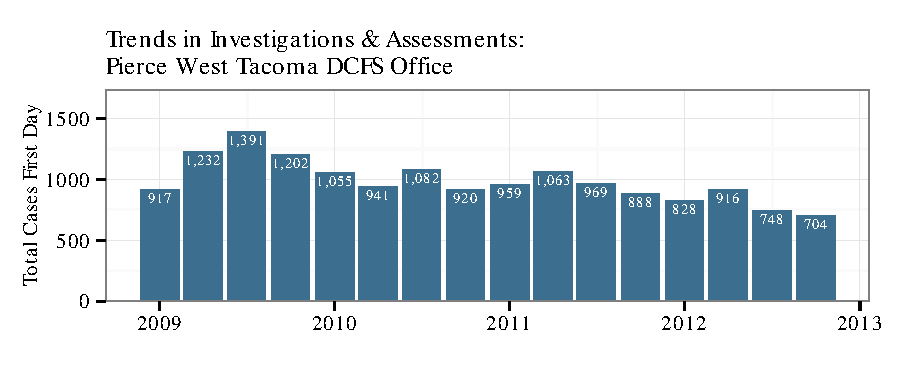
\includegraphics[width=\maxwidth]{figure/ia_focus1} 
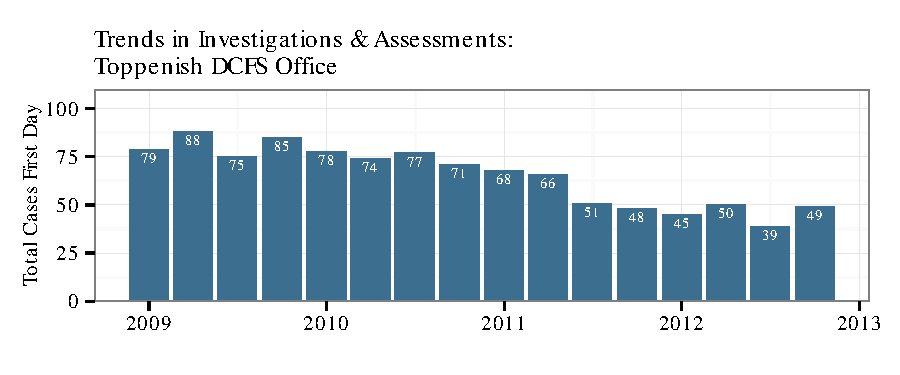
\includegraphics[width=\maxwidth]{figure/ia_focus2} 

}



\end{knitrout}


\subsection{
    \href{http://www.partnersforourchildren.org//child-well-being/visualizations/investigations-assessments/trends}
    {Investigations \& Assessment: Regional Context}
}
To give context to the trend data above, this plot shows the rate of Investigations \& Assessments (as a rate per 1,000 households) in the last quarter for the whole region.

\begin{knitrout}
\definecolor{shadecolor}{rgb}{0.969, 0.969, 0.969}\color{fgcolor}

{\centering 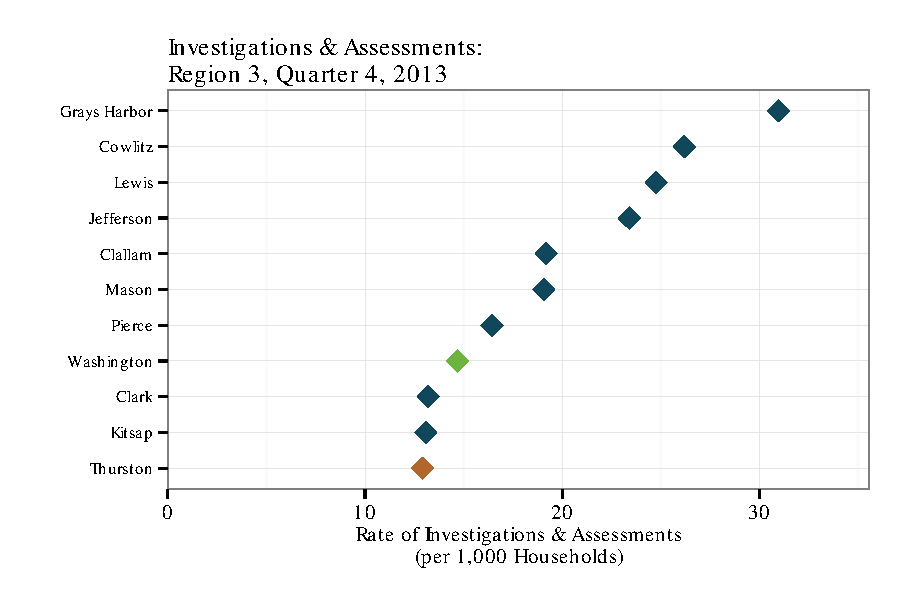
\includegraphics[width=\maxwidth]{figure/ia_context} 

}



\end{knitrout}



%%%%%%%%%%%%%%%%%%%%%%%%%%%%%%%%%%%%%%%%%%%%%%%%
\section{\href{http://www.partnersforourchildren.org/child-well-being/visualizations/home-services/trends}
    {In-Home Services}
}
When an investigation or assessment identifies threats to a child's safety, social workers will first attempt to address the safety threat in the family home when the child's safety can be assured through a safety plan. Various supports are provided to families receiving in-home services. These supports range from concrete support (e.g., food, appliance repair, etc.) to referrals to community services (e.g., drug and alcohol assessments, etc.).

The measurements in this section provide an overview of the population of families receiving in-home services and how the
population of families has changed over time.

\subsection{\href{http://www.partnersforourchildren.org/child-well-being/visualizations/home-services/trends}
    {In-Home Services: Pierce County Focus}
}
These graphs show the recent trends in In-Home Services for all the DCFS offices in
Pierce County.

\begin{knitrout}
\definecolor{shadecolor}{rgb}{0.969, 0.969, 0.969}\color{fgcolor}

{\centering 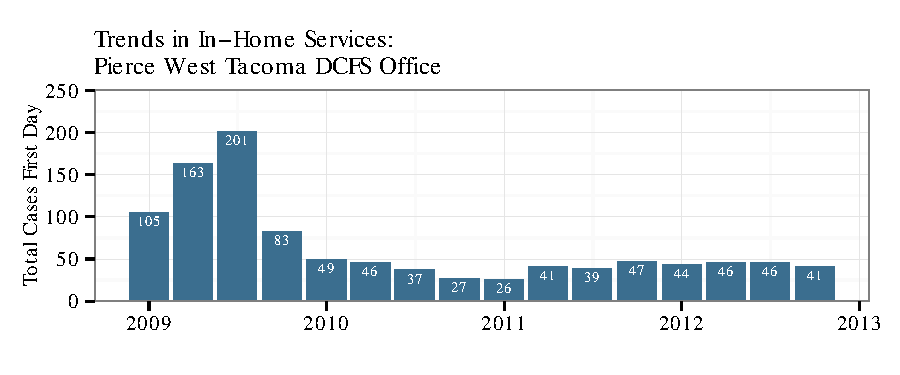
\includegraphics[width=\maxwidth]{figure/ihs_focus1} 
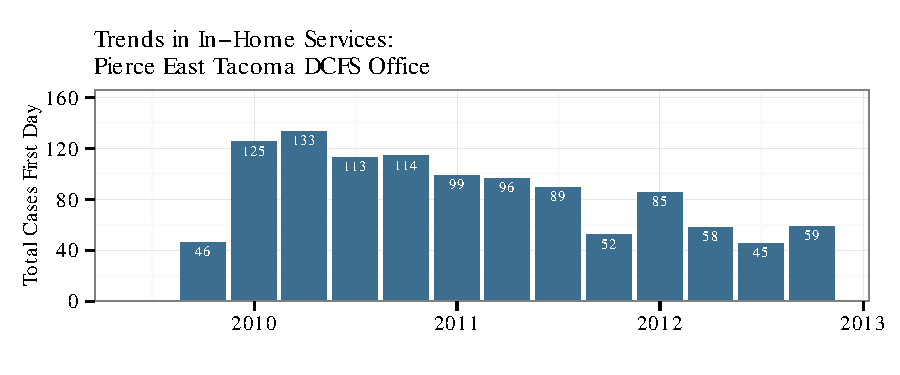
\includegraphics[width=\maxwidth]{figure/ihs_focus2} 

}



\end{knitrout}



\subsection{\href{http://www.partnersforourchildren.org/child-well-being/visualizations/home-services/trends}
    {In-Home Services: Regional Context}
}
To give context to the trend data above, this plot shows the rate of In-Home Services (as a rate per 1,000 households) in the last quarter for the whole region.

\begin{knitrout}
\definecolor{shadecolor}{rgb}{0.969, 0.969, 0.969}\color{fgcolor}

{\centering 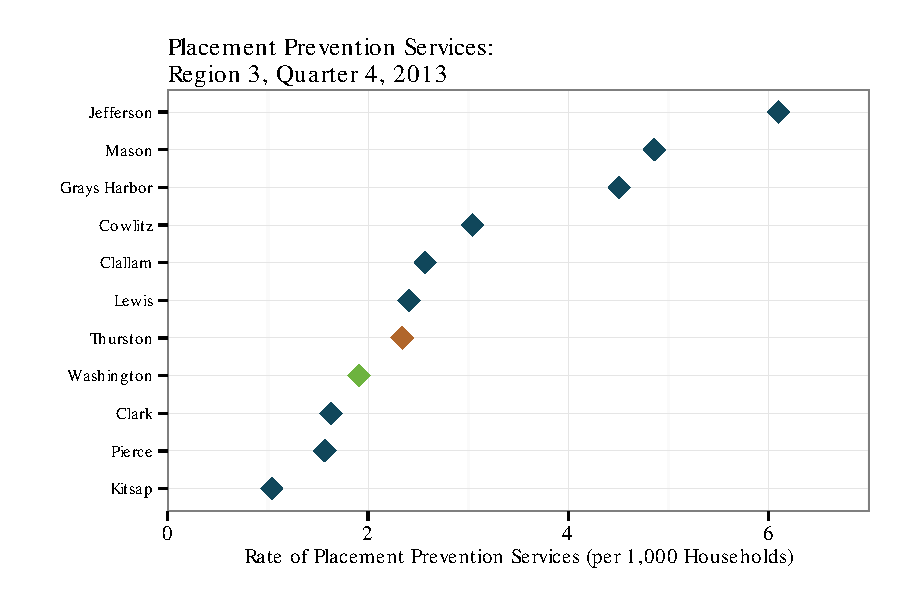
\includegraphics[width=\maxwidth]{figure/ihs_context} 

}



\end{knitrout}



\subsection{\href{http://www.partnersforourchildren.org/child-well-being/visualizations/home-services/safety}
    {In-Home Services: Safety}
}
Sometimes the services provided to families through in-home services do not adequately address the issues identified during the investigation. Other times, new issues are raised during the course of an in-home services case. Sometimes these issues are so significant that the social worker decides that it is not possible for the child to remain safely in their home and takes steps to place the child in out-of-home care.

The measurements in this section identify the timing of placement into out-of-home care among families and their children receiving in-home services during a specified period of time.

% latex table generated in R 3.0.0 by xtable 1.7-1 package
% Fri Apr 12 12:28:08 2013
\begin{table}[ht]
\centering
\caption{Percent of In-Home Service cases resulting in Out-of-Home Care placement.} 
\begin{tabular}{lll}
  \toprule
Office & Within 1 Year & Within 2 Years \\ 
  \midrule
Washington State & 18\% & 20\% \\ 
  Pierce West Tacoma & 21\% & 25\% \\ 
  Pierce East Tacoma & 23\% & 24\% \\ 
   \bottomrule
\end{tabular}
\end{table}



\subsubsection{Interpreting the table}
Generally, lower percentages are better. If in-home services are completely effective, the need to place the a child in out-of-home care should be 

%%%%%%%%%%%%%%%%%%%%%%%%%%%%%%%%%%%%%%%%%%%%%%%%%
\section{\href{http://www.partnersforourchildren.org/child-well-being/visualizations/out-home-care/trends}
    {Out-of-Home Care}
}
When children cannot remain safely in their home, they are placed in out-of-home care. Once a child is placed in out-of-home care, the child welfare system works to place the child in a safe and permanent home. Most children ultimately reunify with their parents after the safety threats have been controlled.
However, some children exit to other permanency outcomes (e.g., adoption, guardianship, etc.).

The measurements in this section provide an overview of the population of children in out-of-home care and how that population has changed over time.

\subsection{\href{http://www.partnersforourchildren.org/child-well-being/visualizations/out-home-care/trends}
{Pierce County Focus}
}
This graph shows the recent trends in Out-of-Home Care for
Pierce County. Most counties maintain a relatively stable out-of-home care population, though smaller counties experience greater volatility (from a percent standpoint).

\begin{knitrout}
\definecolor{shadecolor}{rgb}{0.969, 0.969, 0.969}\color{fgcolor}

{\centering 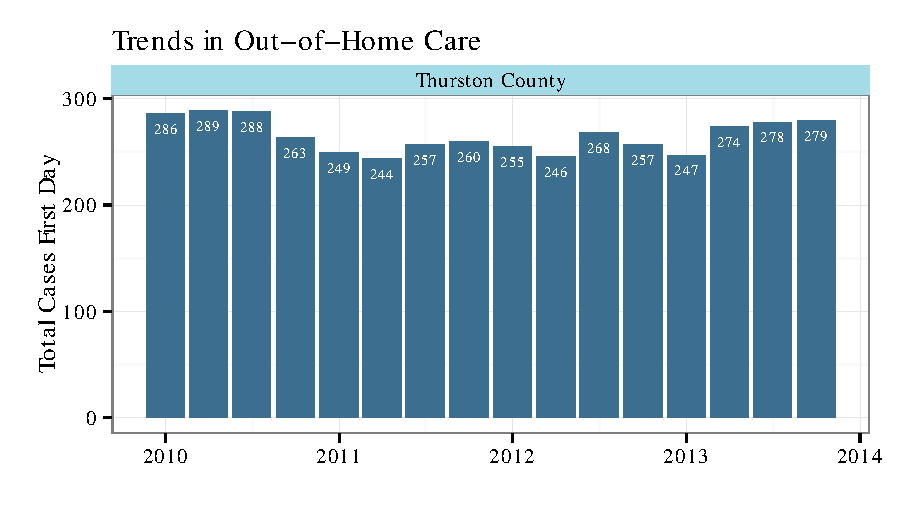
\includegraphics[width=\maxwidth]{figure/ooh_focus} 

}



\end{knitrout}


\subsection{\href{http://www.partnersforourchildren.org/child-well-being/visualizations/out-home-care/trends}
    {Regional Context}
}
To give context to the trend data above, this plot shows the rate of Out-of-Home Care (as a rate per 1,000 children) in the last quarter for the whole region.

\begin{knitrout}
\definecolor{shadecolor}{rgb}{0.969, 0.969, 0.969}\color{fgcolor}

{\centering 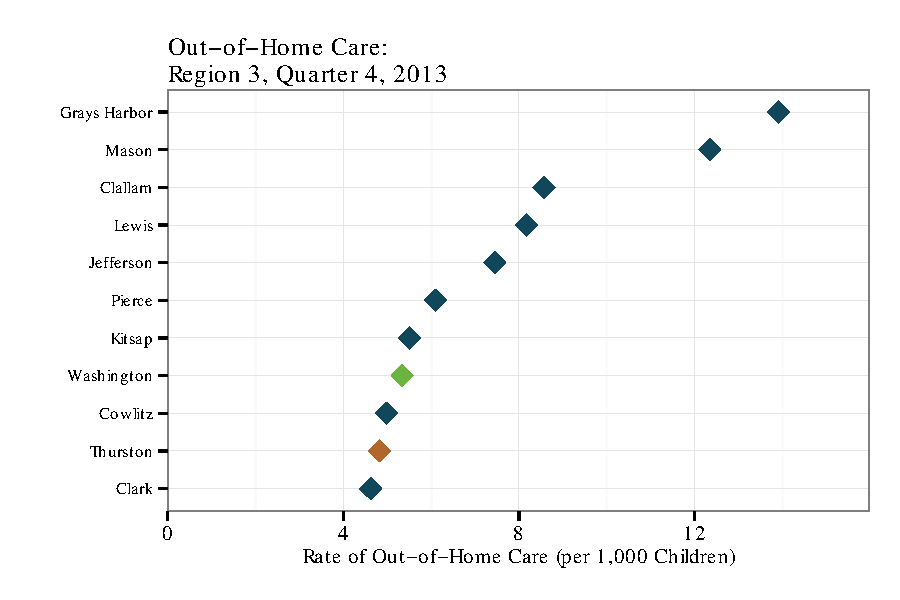
\includegraphics[width=\maxwidth]{figure/ooh_context} 

}



\end{knitrout}


\subsection{\href{http://www.partnersforourchildren.org/child-well-being/visualizations/out-home-care/safety}
    {Safety in Out-of-Home Care}
}

Sometimes when children experience a given permanency outcome (e.g., reunification, guardianship, adoption), safety concerns resurface in the child's home. In certain circumstances, these safety concerns are severe enough that the child needs to re-enter out-of-home care.

The table in this section identifies the percentage of children re-entering out-of-home care within two years of discharge, by discharge type, for all of the counties in Region 3, as well as the Washington state overall. Lower numbers are good, indicating that 

% latex table generated in R 3.0.0 by xtable 1.7-1 package
% Fri Apr 12 12:28:08 2013
\begin{table}[ht]
\centering
\caption{Percentage of children re-entering out-of-home care within 2 years of discharge, by type of discharge. (Blanks indicate that no children in the cohort exited to that discharge type.)} 
\begin{tabular}{llll}
  \toprule
County & Reunification & Adoption & Guardianship \\ 
  \midrule
Skamania & 42.9\% & 0\% &  \\ 
  Jefferson & 37.5\% & 0\% & 0\% \\ 
  Clallam & 31.8\% & 0\% & 0\% \\ 
  Thurston & 22.2\% & 1.9\% & 11.1\% \\ 
  Pacific & 16.7\% & 0\% & 0\% \\ 
  Grays Harbor & 15\% & 0\% & 0\% \\ 
  Pierce & 13.2\% & 2.1\% & 1.1\% \\ 
  Clark & 13.1\% & 1.8\% & 4.3\% \\ 
  Washington State & 12.8\% & 1.5\% & 5.7\% \\ 
  Kitsap & 9.7\% & 0\% & 27.3\% \\ 
  Mason & 8.8\% & 0\% & 0\% \\ 
  Cowlitz & 6.9\% & 0\% & 0\% \\ 
  Lewis & 6.5\% & 0\% & 33.3\% \\ 
  Wahkiakum & 0\% &  &  \\ 
   \bottomrule
\end{tabular}
\end{table}




%% Permanency Chunk
\end{document}
